% temp file for CHapt 08 material 

\begin{ExampleSmall}
Find the system type for a CLNFS consisting of the following elements:


 \[
 C(s) = \frac{500}{s(s+10)} \qquad P(s) = \frac{(s+0.1)}{s(s^2+50s+1500)} \qquad H(s) = 1
 \]
 
 \vspace{0.25in}
 
The combined system $CPH(s)$ has {\bf two} poles at the origin so it is of {\bf type 2}.
\end{ExampleSmall}

 





%\end{frame}  %%%%%%%%%%%%%%%%%%%%%%%%%%%%%%%%%%%%%%%%%%%%%%%%%%%%%%%%%%%%

\subsection{Steady State Error Derivation}

The key to computation of steady state error is the Final Value Theorem of basic Laplace Tranform theory:

\bq\label{FVTheorem}
\lim_{t\to\infty} f(t) = \lim_{s\to 0} sF(s)
\eq

The quantity on the left is the steady state error, after all transient terms have died out.   The Final Value Theorem says we can find this final SSE by evaluating the limit on the right.  However, this theorem only applies if the limit on the left actually exists.  For example, if $f(t) = \sin(\omega t)$, then the limit does not exist.  Looked at in the complex plain, the poles of $F(s)$ must be in the left half plane so that all transients die out. 

Now let's apply the FVT to error.
\[
E(s) = X(s) - C(s)P(s)H(s)E(s)
\]
abbreviating $G(s) = C(s)P(s)$, and simplifying
\[
E(s) \left( 1+GH \right) = X(s)
\]

\bq\label{ErrorResult}
E(s) = \frac {X(s)} {1+GH}  
\eq

Let's apply this result to a specific system where:
\[
C = 10 \qquad P = \frac{50}{s+10} \qquad H = 1 \qquad X(s) = \frac{A}{s}
\]
Note that we have chosen a specific input (step function with amplitude A), for this analysis. 

Using the FVT of Equation \ref{FVTheorem},  Applying Equation \ref{ErrorResult},
\[
E(s) = \frac{A/s}{(1+500/(s+10))} = \frac{A(s+10)}{s(s+10+500)}= \frac{A(s+10)}{s^2+510s} 
\]
Applying the FVT:
\[
\lim_{t\to\infty} e(t) = \lim_{s\to 0} s\frac{A(s+10)}{s^2+510s} = \lim_{s\to 0} \frac{A(s+10}{s+510} = \frac{10A}{510}
\]

\[
\lim_{t\to\infty} e(t) =  0.02A
\]
In other words the Steady State Error (SSE) is 2\%.



%%%%** Section 1.4
\subsection{Steady State Error Examples} 

The following examples illustrate some key properties of steady state error. 

\begin{ExampleSmall}
\[
C = 10 \qquad P = \frac{50}{s+10} \qquad H = 1 \qquad x(t) = Bt \qquad X(s) = \frac{B}{s^2}
\]
This is the same as above, but the input is now a ramp.

\[
E(s) = \frac{B/s^2}{(1+500/(s+10))} = \frac{B(s+10)}{s^2(s+10+500)}= \frac{B(s+10)}{s^3+510s^2} 
\]
Applying the FVT:
\[
\lim_{t\to\infty} e(t) = \lim_{s\to 0} s\frac{B(s+10)}{s^3+510s^2} = \lim_{s\to 0} \frac{B(s+10}{s^2+510s} = \infty
\]
The system is the same, but with a ramp input the steady state error is infinite!

\end{ExampleSmall}



\begin{ExampleSmall}\label{ExIntwRamp}

\[
C = \frac{10}{s} \qquad P = \frac{50}{s+10} \qquad H = 1 \qquad x(t) = Au(t) \qquad X(s) = \frac{A}{s}
\]
This is the same as the first example, but the controller, $C(s)$, now adds a pole at the origin.
 \[
E(s) = \frac{A/s}{(1+500/(s(s+10)))} = \frac{A(s^2+10s)}{s(s^2+10s+500)} 
\]
Applying the FVT:
\[
\lim_{t\to\infty} e(t) = \lim_{s\to 0} \frac{A(s^2+10s)}{s^2+10s+500} = 0
\]

The plant was the same, but by adding a pole at the  origin to the controller, we have eliminated SSE for step input to zero. 
Since this is such a nice result it is worth a look at this new controller Figure \ref{SimpleIntegralController}. 
This controller can be implemented by building an integrator.  Two ways to implement an integrator are an analog op-amp circuit with a feedback capacitor, and a software loop in a microcontroller which sums the difference between input and output. 

\end{ExampleSmall}


\begin{figure}\centering
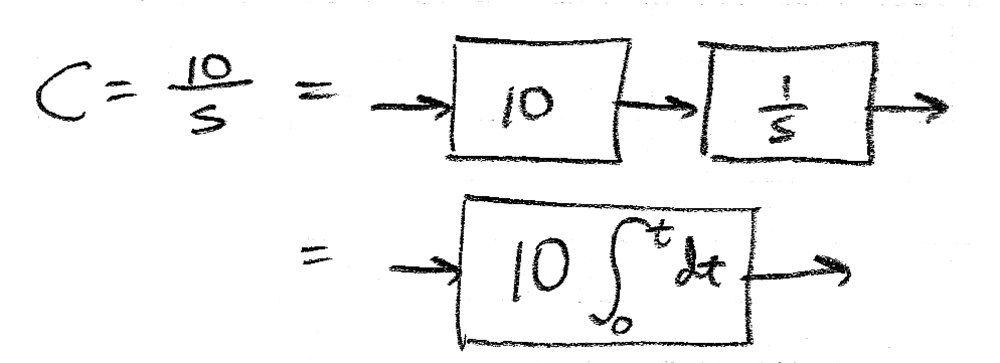
\includegraphics[width=2.5in]{figs08/00786.png}
\caption{A simple controller which has a single pole at the origin can be called an {\it Integral controller}}\label{SimpleIntegralController}
\end{figure}
 
 
 
 
 
 
 
 
 
 
\begin{ExampleSmall}\label{ExIntegwithRamp}
\[
C = \frac{10}{s} \qquad P = \frac{50}{s+10} \qquad H = 1 \qquad x(t) = Bt \qquad X(s) = \frac{B}{s^2}
\]
This is the same as Example \thechapter.\ref{ExIntwRamp}, but the input is now a ramp.

\[
E(s) = \frac{B(s^2+10s)}{s^2(s^2+10s+500)} 
\]
Applying the FVT:
\[
\mathrm{SSE} = \lim_{s\to 0} \frac{B(s^2+10s)}{s^3+10s^2+500} = \lim_{s\to 0} \frac{B(s+10}{s^2+10s+500} 
\]
\[
= \frac{10}{500}B = 0.02B
\]
With the new controller, we have changed the SSE for ramp input from $\infty$ to 2\%!   Our controller has increased the system type by one and this made a big difference on SSE with the ramp input. 


\end{ExampleSmall}



\subsection{Steady State Error Summary}

We've seen examples of how changing the system type or changing the input can make a big difference in the amount of steady state error.  You might even notice a pattern in the examples above relating the ``input type" (the power of $s$ in the Laplace transform of the input signal) and the system type to the nature of the SSE.  To see this relationship, let's take a closer look at Example \thechapter.\ref{ExIntegwithRamp}. 

Writing out the limit again without canceling any terms, 
\[
\mathrm{SSE} = \lim_{s\to 0} \frac{sBs(s+10)}{s^2(s(s+10)+500} 
\]
We have two $s$'s on the top.  One comes from the final value theorem, and the second one from the denominator of $C(s)$.  On the bottom, we have $s^2$, which comes from the ramp input.    The FVT term and the $C(s)$ denominator term combine to cancel the $s^2$ from the ramp input.   Thus, if the input is 
\[
X(s) = \frac{A}{s^n}
\]
then we need at least $n-1$ poles at the origin in the combined controller and plant (again assuming $H=1$).    


\begin{ExampleSmall}
Now we'll consider a general system with a gain factor, $K$, and $n$ poles at the origin in the controller, as well as a general input,
\[
C = \frac{K}{s^n} \qquad P = \frac{50}{s+10} \qquad H = 1 \qquad x(t) = Bt \qquad X(s) = \frac{D}{s^m}
\]

\[
\mathrm{SSE} = \lim_{s\to 0} \frac{s}{s^m} \frac{D}{\left(1+\frac{K}{s^n}\frac{50}{(s+10)}\right )}
\]

\[
\lim_{s\to 0} \frac{1}{s^{m-1)} \frac {Ds^N(s+10)} {(s^n(s+10)+50K)} = \lim_{s\to 0} \frac{Ds^n(s+10)} {s^{n+m}+10s^{n+m-1} + 50Ks^{m-1}}
\]

\end{ExampleSmall}


For this limit to be finite as $s\to 0$, we need to have no remaining powers of $s$ in the denominator after cancelation.  Thus  if
\[
n > m-1
\]
the error if zero.   If $n=m-1$ we have after cancellation
\[
\mathrm{SSE} = \lim_{s\to 0} \frac  {Ds^n(s+10}   {s^{2n-1} + 10s^{2n-2} + 50ks^n} = \frac {10D}  {50K}
\] 


All of these relationships can be summed up in Table \ref{SystemTypeError}.    
It is worth remembering that SSE only applies after transients due to the non-zero poles are over.  Such transients are illustrated for some typical situations in Figure \ref{SSEtransients}


%%%%** Figure 2 
\begin{figure}\centering
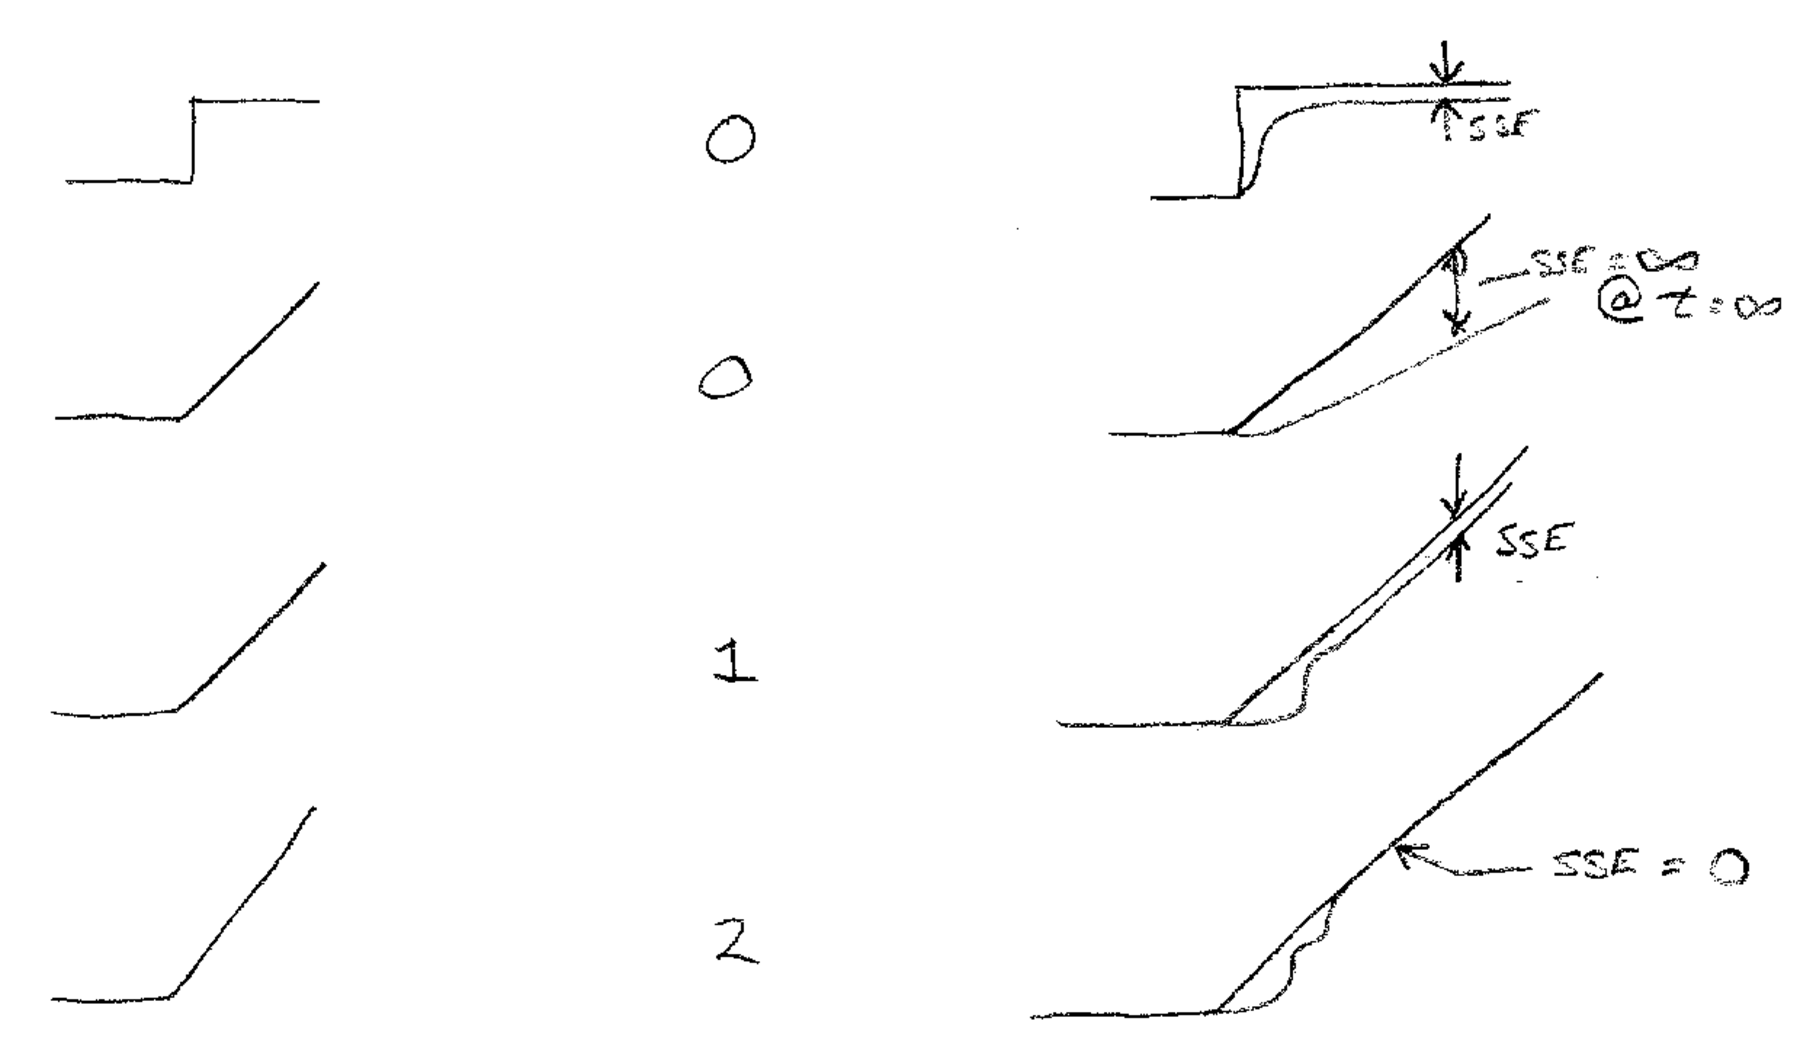
\includegraphics[width=4.50in]{figs10/00476.png}
\caption{Qualitative Illustrations of different SSE and transient responses.}\label{SSEtransients}
\end{figure} 


%\end{frame}


\begin{table}\centering
\begin{tabular}{|c|c|c|c|c|} \hline
Type	&	$C(s)P(s)$	&	Step $(n=1)$	&	Ramp $(n=2)$	& 	Parabola $(n=3)$   \\ \hline
0	&	$K\dots$	&	finite		&	$\infty$	&	$\infty$	   \\ \hline
1	&	$\frac{K}{s}\dots$&	0		&	finite		&	$\infty$	   \\ \hline
2	&	$\frac{K}{s^2}\dots$&0		&       0        	&	finite		   \\ \hline
\end{tabular}

\caption{SSE vs. System Type and Input Type}\label{SystemTypeError}
\end{table}


%%%%%%%%%%%%%%%%%%%%%%%%%%%%%%%%%%%%%%%%%%%%%%%%%%%%%%%%%%%%%%%%%%%%%%%%%%%%%%%%%%%%%%%%%%%%%%%%%%%%%%%%%%%


\section{Time Domain Performance of 2nd Order Systems}
%\begin{frame}
%\frametitle{Time Domain Performance}


%%%%** Figure 3 
\begin{figure}\centering
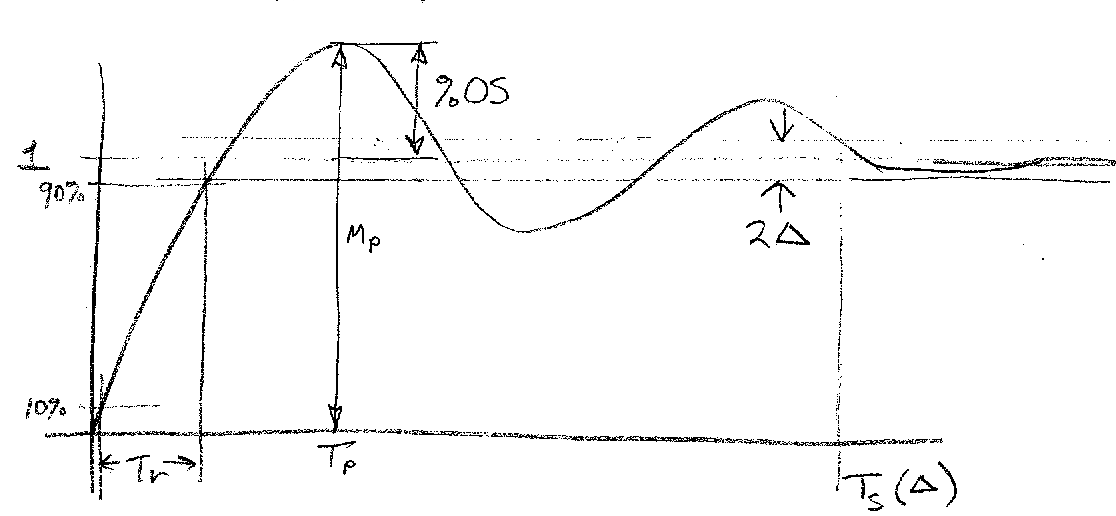
\includegraphics[width=4.0in]{figs10/00472.png}
\caption{A step response with labels for percent overshoot (\%OS) and settling time, $T_S$.}\label{stepresponse}
\end{figure}
 


 The performance of second order systems (systems having 2 poles) is fairly easy to characterize.  We develop intuition about the relationship of pole locations to time response from second order systems.  Practical systems are usually higher order  and we use computation for them.	%<*h>

%\end{frame}
%\begin{frame}


	%<*>
\begin{itemize}
	\item Settling Time: $T_s$: time to get within 2\% of final value
	\item $T_s \approx \frac{-4}{\sigma}$ (derived in books) \\
$\sigma$ is real part of poles.
	\item \%OS = percent overshoot  (computed numerically)
	\item 
	\begin{tabular}{c|c|c}
	\%OS	& $\zeta$	& $\theta$	\\\hline   
	10\%	& 0.587		& 54$^\circ$	\\
	 5\%	& 0.695		& 46$^\circ$	\\
	 2\%	& 0.777		& 39$^\circ$	\\
	 1\%	& 0.829		& 34$^\circ$	\\
	\end{tabular} 
\end{itemize}


%\end{frame}
%\begin{frame}



 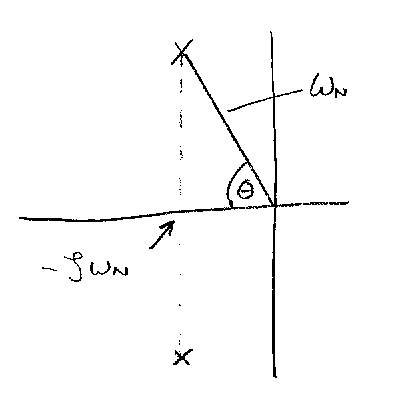
\includegraphics[width=1.5in]{figs10/00478.png}

 
  $\zeta =$ damping ratio.   $\theta$ = s-plane angle. \\[0.25in]

 
%\end{frame}  %%%%%%%%%%%%%%%%%%%%%%%%%%%%%%%%%%%%%%%%%%%%%%%%%%%%%%%%%%%%
 

%%%%** Section 1.6
\subsection{S-plane Regions}


%\begin{frame}
%\frametitle{S-Plane Regions}

Each performance spec corresponds to a specific region of the $s$-plane which is illustrated in Figure \ref{splaneregion}:

\begin{tabular}{ll}
$T_s$:  Vertical line at $\sigma = -4/T_s$.     &
Left of line:   faster,  \\ & Right of line, slower
\\
\%OS:  Wedge at $\theta= \pm \cos^{-1}(\zeta)$.  &
Right of lines:  More overshoot, \\ & Left of lines, less overshoot.
\end{tabular}


%\end{frame}
%\begin{frame}
 
Example: $T_s \leq 2\mathrm{sec}$, \%OS $\leq 5$%


%%%%** Figure 4 
\begin{figure}\centering
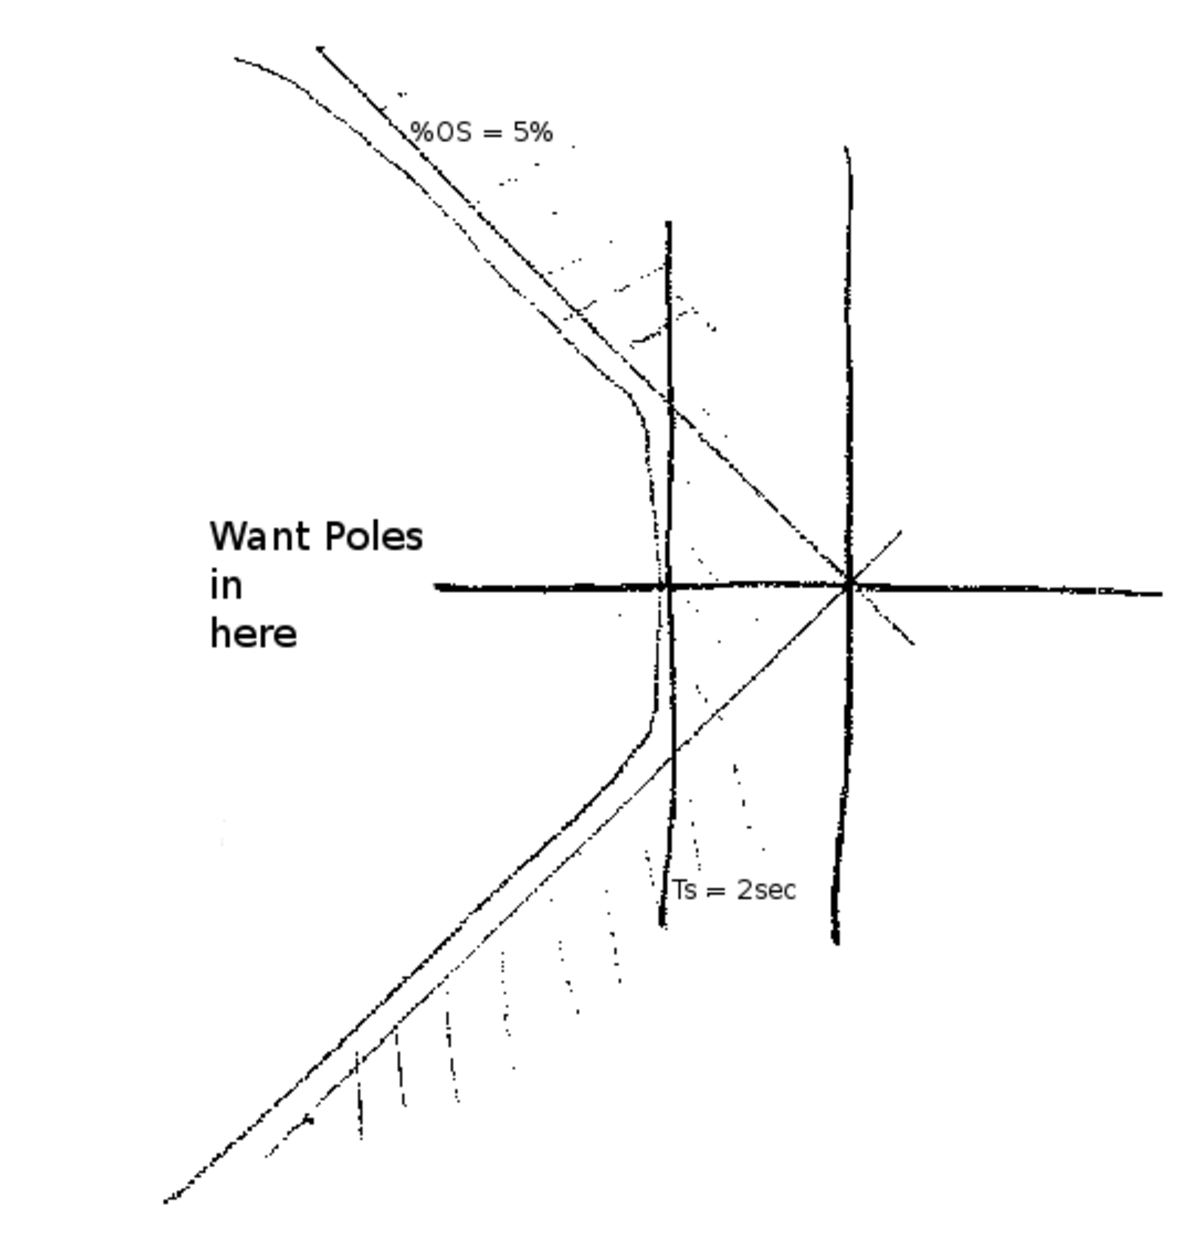
\includegraphics[width=3.0in]{figs10/00473.png}
\caption{Any poles in the region shown will meet or exceed the specs: \%OS = 5\% and $T_S<=$2ms.}\label{splaneregion}
\end{figure}





%%%%%%%%%%%%%%%%%%%%%%%%%%%%%%%%%%%%%%%%%%%%%%%%%%%%%%%%%%%%%%%%%%%%%%%%%%%%%%%%%%%%%   PID Control


\section{PID Controller}
	%<*>
%%%%** Section 1.11
\subsection{Closed Loop Design Problem} 

%\begin{frame}
\begin{itemize}

	\item Plant: $P(s)$

	\item Controller: $C(s)$

	\item Closed Loop Response:   $\frac{C(s)P(s)}{1 + C(s)P(s)}$

	\item {\bf Design problem: }
           Specify Controller/Compensator $C(s)$ to improve step response compared to open loop system, $P(s)$.
\end{itemize} 
 
%\end{frame}  %%%%%%%%%%%%%%%%%%%%%%%%%%%%%%%%%%%%%%%%%%%%%%



%%%%** Section 1.12
\subsection{PID Control} 

%\begin{frame}
%\frametitle{PID Control}
%%%%** Figure 6 
\begin{figure}\centering
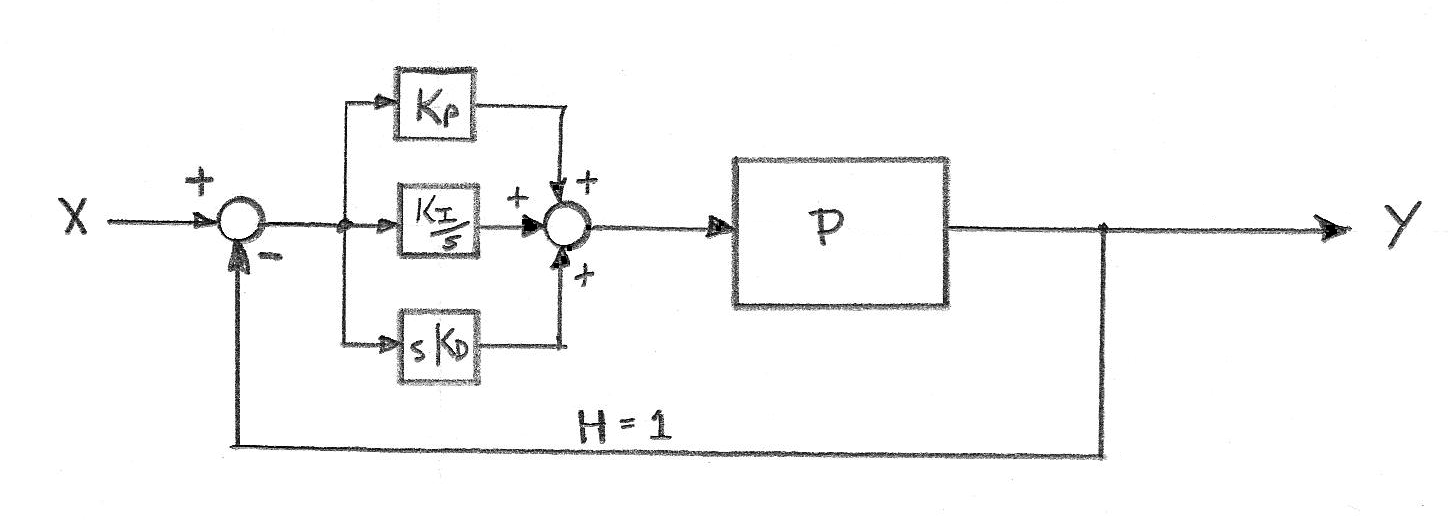
\includegraphics[width=4.0in]{figs10/00651.png}
\caption{The PID controller.}\label{PIDBlockDiagram}
\end{figure}

%\end{frame} %%%%%%%%%%%%%%%%%%%%%%%%%%%%%%%%%%%%%%%%%%%%%%%%%%%%%%

%\begin{frame}
\begin{itemize}
	\item Most common controller in industry BY FAR
	\item
$C(s) = \frac{Ks+K_Ds^2 + K_i}{s} = \frac{K_D(s^2 + \frac{K}{K_D}s+ \frac{K_i}{K_D})}{s} =
\frac{K_D(s+z_1)(s+z_2)}{s}$
	\item 0,1, or 2 zeros,  for designer to place, plus one pole at $s=0$
	\item Zeros:   Help stability, improve transient response
	\item Pole at origin:  improve steady state error.
\end{itemize}
 

%\end{frame} %%%%%%%%%%%%%%%%%%%%%%%%%%%%%%%%%%%%%%%%%%%%%%%%%%%%%%


%%%%** Section 1.13
\subsection{Basics}

%\begin{frame}
%\frametitle{Basics}

The PID controller is

\begin{equation}\label{PID}
C_{PID}(s) = K_P + \frac{K_I}{s} + K_Ds = \frac{K_Ps+K_i + K_Ds^2}{s} = \frac{K_D(s^2 + \frac{K_P}{K_D}s + \frac{K_I}{K_D})}{s}
\end{equation}

%\end{frame} %%%%%%%%%%%%%%%%%%%%%%%%%%%%%%%%%%%%%%%%%%%%%%%%%%%%%%



%\begin{frame}
{\bf $K_P$}  is the proportional gain.
Looking at the second term above, you can see that $K_P$ directly multiplies the error (the input to the controller).  If the other gains were zero, the control output, $u$, will be  linearly proportional to error.	%<h>

\[
u(t) = K_P e(t)
\]

%\end{frame} %%%%%%%%%%%%%%%%%%%%%%%%%%%%%%%%%%%%%%%%%%%%%%%%%%%%%%



%\begin{frame}
{\bf $K_I$} is the integral gain.
Looking at the second term above we see that $K_I$ appears multiplied by $1/s$, the integral operator.  If the other gains were zero, the control output, $u$, would be $K_I$ times the time integral of the error:	%<h>

\[
u(t) = K_I \int_0^t e(t) dt
\]



%\end{frame} %%%%%%%%%%%%%%%%%%%%%%%%%%%%%%%%%%%%%%%%%%%%%%%%%%%%%%



%\begin{frame}
{\bf $K_D$} is the derivative gain.
Looking at the second term above we see that $K_D$ appears multiplied by $s$, the derivative operator.  If the other gains were zero, the control output, $u$, would be $K_D$ times the time derivative of the error:	%<h>

\[
u(t) = K_D \frac{d}{dt}e(t)
\]
In fact, using the inverse Laplace transform we can write:
\[
u(t) = K_P e(t)  + K_I \int_0^t e(t) dt + K_D \frac{d}{dt}e(t)
\]
 

	%<*>


%\end{frame} %%%%%%%%%%%%%%%%%%%%%%%%%%%%%%%%%%%%%%%%%%%%%%%%%%%%%%



%%%%** Section 1.14
\subsection{Simulation of PID controllers}

	%<*h>
Looking again at equation (\ref{PID}), we can see from the far right hand side that the PID controller has two zeros and one pole.   Such a system cannot be physically realized and is called {\it improper}.   Often this condition is ignored because the plant has enough poles to make the overall forward path ($C(s)P(s)$) proper.  However, what if you would like to make and sell a PID controller box (Figure \ref{pidbox}).
 
 
We also have this problem because we define the controller in our script as a separate system and Scilab cannot simulate an improper system.
To fix this we simply add another pole to the PID controller at a high enough frequency so that it does not affect our response.  This imediately raises two questions


%  Solution:  Add another high frequency pole:  $\frac{a}{(s+a)}$


\begin{enumerate}
  \item Why doesn't a high frequency pole affect the system?
  \item How high is ``high enough"?
\end{enumerate}

%\end{frame} %%%%%%%%%%%%%%%%%%%%%%%%%%%%%%%%%%%%%%%%%%%%%%%%%%%%%%%%%%%%%%%%%%
 



%\begin{frame}

For question one, consider the Bode plot of the basic one-pole system	%<h>

%\frametitle{Q1:  Why doesn't it effect the system?}

\[
P(s) = \rho/(s+\rho)
\]

for $\omega << \rho$, $P(j\omega) = 1$.
Thus for frequencies substantially below $\rho$, $P(s)$ has no effect.	%<h>

%\end{frame} %%%%%%%%%%%%%%%%%%%%%%%%%%%%%%%%%%%%%%%%%%%%%%%%%%%%%%%%%%%%%%%%%%




%\begin{frame}
%\frametitle{Q2: How high is ``high enough"?}

For question two, let us set $\rho$ 10 times higher than the highest pole or zero of our system.   Technically we should know the zeros of the PID controller to do this, but if we {\it assume} that the zeros of a good controller will be in the neighborhood of the poles of the plant, then 10 times greater than the highest frequency plant pole/zero will also be far from the PID controller zeros.	%<h>

$\rho = 10\times pz_{max}$	%<sh>

where $pz_{max}$ is the highest pole or zero in the system.	%<h>

Thus we will add a pole, $\rho$,  to the PID controller in our simulations as follows:	%<h>
 
% \begin{equation}\label{PID2}
\[
C_{PID2}(s) = \frac{\rho(K_Ps+K_i + K_Ds^2)}{s(s+\rho)} = \frac{\rho K_D(s^2 + \frac{K_P}{K_D}s + \frac{K_I}{K_D})}{s(s+\rho)}
\]
% \end{equation}

Now $C_{PID2}$ is proper
because it has the same number of poles and zeros, two.  Thus, Scilab can simulate it and it is also physically realizable.	%<h>








%%%%%%%%%%%%%%%%%%%%%%%%%%%%%%%%%%%%%%%%%%%%%%%%%%%%%%%%%%%%%%%%%%%%%%%%%%%%%%%%%%%%%%%%%%%%%%%%%%%     Control Effort

%%%%** Section 1.15
\subsection{Control Effort}\label{CtlEff}

%\begin{frame}                                                                                                                                                                                                                                                                               
%\frametitle{Control Effort}

Control effort is the level of output needed by the controller to achieve the step response.  All other things being equal, a controller which achives the specs with lower control effort is better.  Often there is a limited maximum effort that a given system can output.  For example, a DC motor has a maximum torque that it is capable of. In this case, it is meaningless to have a settling time that is very fast if that requires 10 times more torque that the motor has available.  Often, controller gains can be found to meet {\bf any} $T_S$ and $\%OS$ spec if control effort limits are ignored.	%<h>

% ``Control Effort", $U$,  = output of controller (into plant)

Computing control effort is easy.  Consider the system below which has a controller, plant and feedback.	%<h>

%\end{frame}  %%%%%%%%%%%%%%%%%%%%%%%%%%%%%%%%%%%%%%%%%%%%%%%%%%%%
 

%\begin{frame}



%%%%** Figure 8 
\begin{figure}\centering
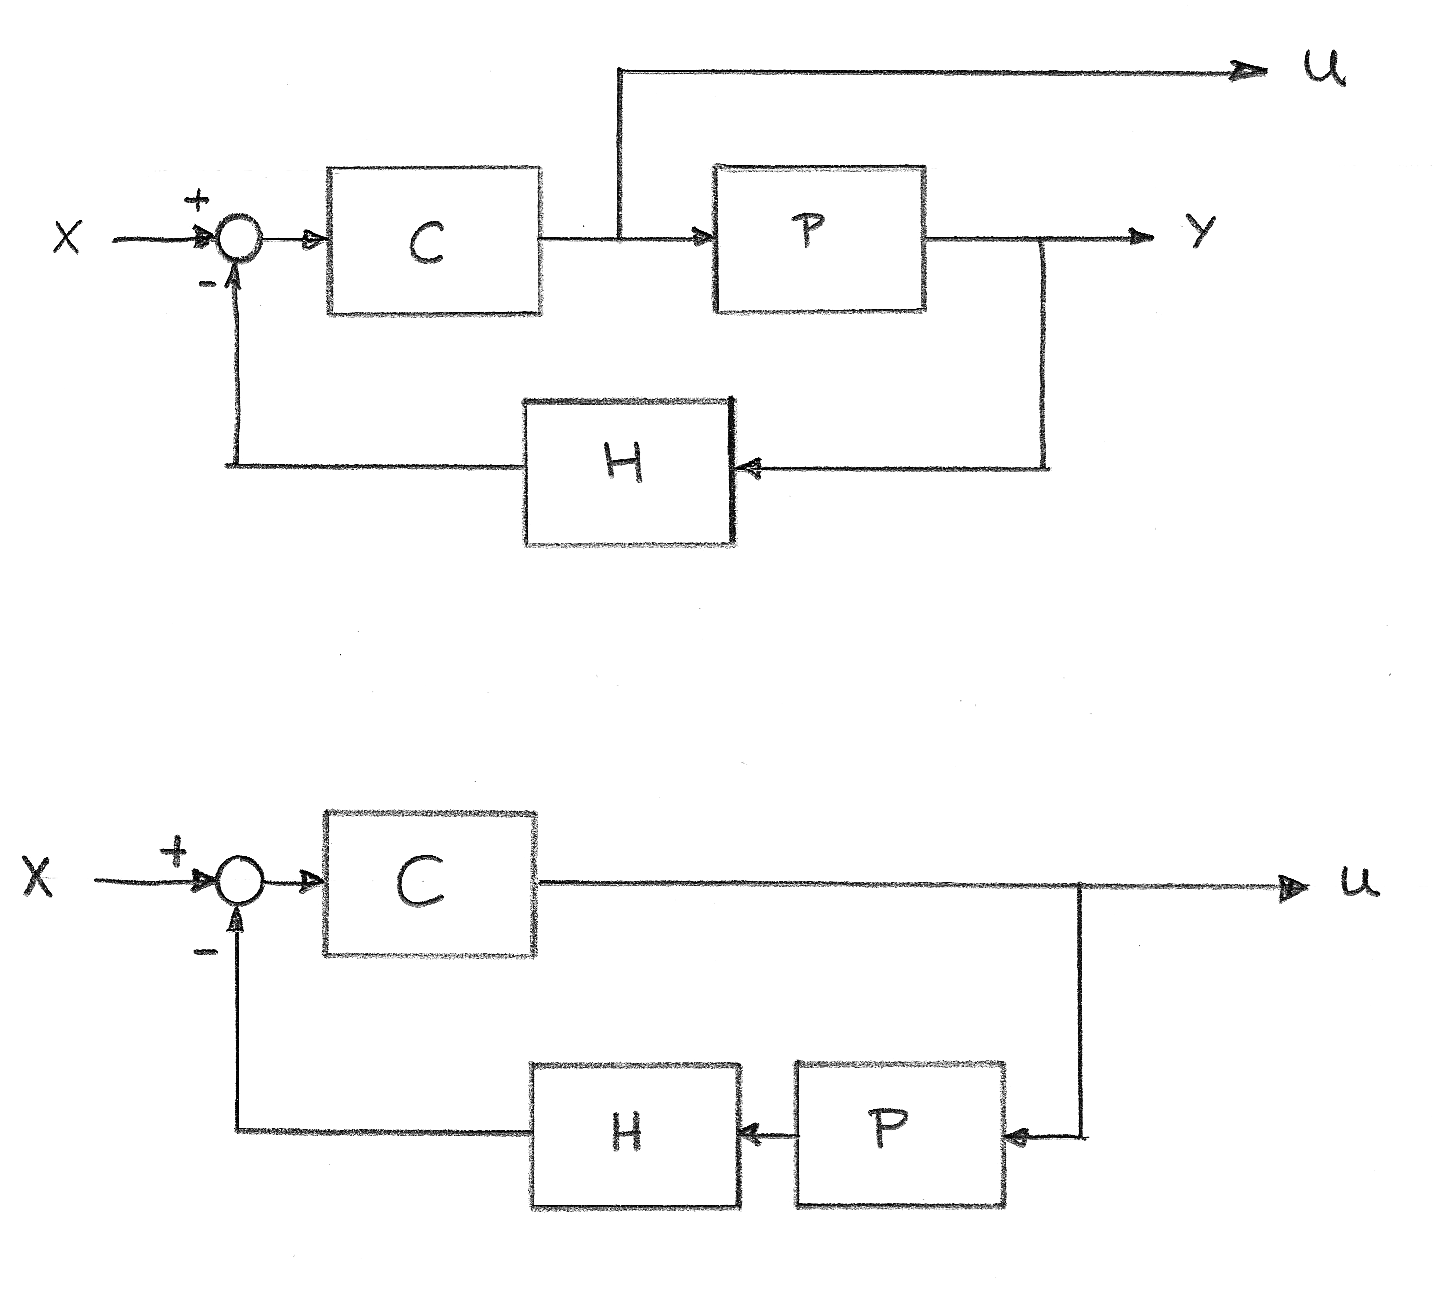
\includegraphics[width=75mm]{figs10/00650.png}
\caption{Control effort signal $u(t)$ or $U(s)$ comes from the output of the controller. We can easily get U by simulating the bottom system.}\label{controleffort}
\end{figure}



%\end{frame}  %%%%%%%%%%%%%%%%%%%%%%%%%%%%%%%%%%%%%%%%%%%%%%%%%%%%



%\begin{frame}
The top system looks conventional, except we have brought out the control effort signal.   In the second system we have simply rearranged the blocks without changing any connections.   However we can now see this as a new feedback system having feedforward path $C$ and feedback $PH$.  Giving the traditional name  $U$ to the control output,	%<h>
\[
\frac{U(s)}{X(s)} = \frac {C(s)}  {1+C(s)P(s)H(s)}
\]

%\end{frame}  %%%%%%%%%%%%%%%%%%%%%%%%%%%%%%%%%%%%%%%%%%%%%%%%%%%%


%\begin{frame}
%\frametitle{Control Effort Metrics}
If we have a limit on our actuator, for example,	%<h>
\[
\tau_{max} = 1.5 NM
\]
then an appropriate measure of performance would be the maximum value of $u(t)$: does it exceed 1.5$NM$? .   On the other hand, if we are concerned with total energy consumption, an appropriate measure might be	%<h>
\[
\int_0^{Tmax} u^2(t) dt
\]
where $T_{max}$ defines a time window that makes sense for our application.	%<h>


%\end{frame}  %%%%%%%%%%%%%%%%%%%%%%%%%%%%%%%%%%%%%%%%%%%%%%%%%%%%








\section{Manual Design of PID controller}
% \section{}

In this section we will design PID control gains through a ``manual" method.  Specifically we will find the values of $K_P, K_I, K_D$ for a given plant and a set of performance specifications, including control effort.  Although this method uses the computer to speed Root Locus plotting, it is designed to give a starting point for more accurate design methods discussed below in which 
we will rely on computerized search-based optimization to design controller parameters.  

Although the optimization search is effective and can take more performance criteria into account, the search can go significantly faster with an initial starting guess.   Unfortunately there is no ``typical" range of PID parameter values which could be used as a standard starting range.  

Although manual design of PID controllers is possible (see most of the textbooks), there is no reason that we cannot use the computer to speed the manual calculation.   In particular, we will use the root locus command to guide our PID design into roughly the neighborhood where we expect solutions to reside. 



\begin{Example}

We have a large industrial machine with the following plant model:

\[
P(s) = \frac {(s+1)} {(s+2.0)(s+0.7+0.2j)(s+0.7-0.2j)}, \quad H=1
\]
 

Our desired performance specifications are:

\[
T_{SD} = 3.33 sec  \qquad 
\%OS = 10\%        \qquad
SSE_D = 0
\] 

It is decreed that we shall use a PID controller, but we have no initial values for $K_P, K_I, K_D$. 

We will be using the root locus method to analyze performance of PID controllers.  Because we need to plot zeros and poles of the controller,  the most useful form of the PID controller is:
\[
C(s) = \frac{K(s+z_1)(s+z_2)}{s}
\]


{\bf Problem Statement: }  Find values of $K, z_1, z_2$ or equivalently $K_P, K_I, K_D$ that can be reasonably expected to meet the specifications. 


\subsection{Solution method}

\begin{enumerate}
 \item Make the assumption that the two complex conjugate poles closest to the origin are dominant (false!).
 \item Draw the s-plane and draw the region(s) corresponding to the performance specifications.
 \item Plot the poles and zeros of the plant on the s-plane.
 \item Place two zeros in places such that they will ``pull" the root locus through the target region\footnote{Assuming the plant poles do not already meet the specs(!)}. Use Scilab to plot the Root Locus (``{\tt evans(sys)}" command)
  \item If the root locus goes through the target region, use the mouse to find the value of $K$ at the target location.
  \item Use the chosen $z_1, z_2$ and $K$ values to derive  $K_P, K_I, K_D$ (see Section \ref{Kpderive})
  \item If the root locus does NOT go through the target region, go back to step 4 and try again. 
\end{enumerate} 

\end{Example}

\subsection{Deriving $K_P, K_I, K_D$ from controller zeros}\label{Kpderive}

There are several forms of the PID controller including: 
\[
C(s) = K_D \left ( s^2+ \frac{K_P}{K_D}s + \frac{K_I}{K_D} \right ) \frac{1}{s}
\]
Let
\[
PC(s) = \left ( s^2+ \frac{K_P}{K_D}s + \frac{K_I}{K_D} \right )
\].

Suppose that zero locations we like are 
\[
z_i = (s + 1.7 \pm 0.5j)
\]
and that the result of step 5 above yields $K_D = 1.85$.   Multiplying out gives
\[
PC(s) = (s + 1.7 + 0.5j)(s + 1.7 - 0.5j)  = s^2 + 3.4s + 3.14
\]
Therefore,
\[
C(s) = 1.85 PC(s) \frac{1}{s} = 1.85(s^2 + 3.4s + 3.14)\frac{1}{s} 
\]
Giving us
\[
K_P = 3.14\times1.85 = 6.29  \qquad  K_I = 3.4\times 1.85 = 5.81 \qquad K_D = 1.85
\]
This gives us a rough design which should be a good start for the computer optimization process. 

 

% \section{Summary of Notation}